\documentclass[10pt]{article}

\usepackage[T1]{fontenc}
\usepackage[utf8]{inputenc}
\usepackage[english]{babel}
\usepackage{amssymb,amsfonts,amsmath,amsthm}
\usepackage{graphicx}
\usepackage{lmodern}
\usepackage{cases}
\usepackage{pdfpages}
\usepackage[margin=60pt]{geometry}
\usepackage{abstract}
\renewcommand{\abstractnamefont}{\normalfont\Large\bfseries}
\renewcommand{\abstracttextfont}{\normalfont\normalsize}

\usepackage{pgfplots}
%\usepgfplotslibrary{colormaps}
\pgfplotsset{every axis/.append style={line width=1pt}}

\usepackage{multicol}
\usepackage{float}
\floatstyle{boxed}
\newfloat{boxframe}{H}{}
\floatname{boxframe}{Box}

\newcommand{\ud}{{\mathrm{d}}}
\newcommand{\pr}{{\mathbb{P}}}
\newcommand{\nN}{{n_\textrm{H}}}
\newcommand{\nI}{{n_\textrm{I}}}
\newcommand{\Xnema}{\textit{X. nematophila} }
\newcommand{\Scarpo}{\textit{S. carpocapsae} }
\newcommand{\Xenonema}{\textit{Xenorhabdus nematophila} }
\newcommand{\Steincarpo}{\textit{Steinernema carpocapsae} }
\newcommand{\Xeno}{\textit{Xenorhabdus} }
\newcommand{\Stein}{\textit{Steinernema} }
\newcommand{\Photo}{\textit{Photorhabdus} }
\newcommand{\Hetero}{\textit{Heterorhabditis} }
\newcommand{\IBD}{IBD}
\newcommand{\qw}{Q_\mathrm{w}}
\newcommand{\qb}{Q_\mathrm{b}}
\newcommand{\psis}{\psi_\mathrm{s}}
\newcommand{\psic}{\psi_\mathrm{c}}

\author{Latrille Thibault\\
\small thibault.latrille@ens-lyon.fr\\[-0.8ex]}
\title{Phenotypic variation as a cooperative strategy in \Xeno and \Photo} 
\begin{document}
%\includepdf[pages={1}]{first_page.pdf}
\begin{abstract}
Bacteria of the genus \Xeno and \Photo both colonize and influence the behavior of nematodes, \Stein and \Hetero respectively.
The nematodes infect, colonize and ultimately kills off an insect host, with the help of the bacteria. 
Thus the bacteria are symbiotic of two hosts, helping one to reproduce optimally while killing the other. 
Many studies focused on the symbiotic association between the bacteria and their respective hosts, but they scarcely focused on cooperation at the bacterial level. 
We here provide evidence that the parasitic life cycle of these bacteria has a lot of influence on their relatedness, and thus on cooperation between bacteria. 
Cooperative evolutionary strategies of bacteria are investigated in the light of their symbiotic life cycle. 
We here provide ground on the occurrence that phenotypic variation, observed experimentally in both \Xeno and \textit{Photorhabdus}, is a cooperative strategy. 
We provide a very simple equation connecting phenotypic variation to relatedness. The relatedness is subsequently derived as a function of demographic parameters, experimentally accessible.


\smallskip
\noindent \textbf{Keywords.} cooperation, phenotypic variation, \textit{Xenorhabdus}, \Photo
\end{abstract}
\begin{multicols}{2}
\section*{Introduction}
\begin{figure*}[hbt!]
	  \centering
	  \label{fig:life_cycle}
       \includegraphics[width=14.0cm]{Figures/life_cycle.png}\\
		\caption{ \textbf{ The bacteria life cycle.} 
		The infective juvenile nematode containing bacteria (nematode–bacteria complex) enters a susceptible insect host through natural openings that include the mouth, anus and spiracles. 
		After entering the insect blood system, the nematode releases the bacteria. 
		The bacteria undergo an exponential growth until the population reaches approximately $10^9$ bacteria, the growth is followed by a plateau. 
		Together, the nematode and bacteria overcome insect immunity and kill the insect. 
		The insect cadaver is used as a nutrient source and is protected from opportunistic infection and scavenging by metabolites produced by bacteria.  
		Within this environment, nematodes reproduce sexually and progeny develop through four juvenile stages. 
		Some nematodes develop into infective juveniles after being recolonized by their respective bacteria. 
		The pair then exits the depleted insect carcass in search of a new host.}
\end{figure*}
Studies of \Photo and \textit{Xenorhabdus}, closely related $\gamma$-proteobacteria, have significant potential to reveal both common and distinct aspects of pathogenesis and mutualism, as each of these bacteria naturally enter into both types of relationships during their life cycle: they are pathogens of insects and are mutualists of nematodes from the genus \Hetero and \Stein respectively \cite{Herbert2007,Akhurst1982a,Somvanshi2012}. 
For bacteria in the genus \textit{Xenorhabdus}, the bacterium \Xenonema and its host \Steincarpo has been extensively studied experimentally and is consider as a model for the genus. 
Equivalently, in the genus \textit{Photorhabdus}, the species \textit{Photorhabdus luminescens} and its host \textit{Heterorhabditis bacteriophora} has been extensively studied experimentaly. 
Thus, if not specially stated, the experimental results presented are corroborated at the species and not genus level. However the life cycle is common to all species in those genii.

The mutualistic relationship between the bacteria and the nematode is not obligate, as both partners can survive in the absence of the other. 
Thus, aposymbiotic nematodes can be obtained and assessed for responses to diverse bacterial and environmental stimuli. 
However, symbiotic bacteria are required for nematodes to reproduce efficiently during their life cycle \cite{Sicard2003}. 

Nematodes are either found in insect hosts or in the soil (Figure 1). 
The soil-dwelling vector stage, called the infective juvenile (IJ), is encased in a double cuticle, and is non-feeding owing to its closed mouth and anus.
Prior to the IJ stage, ingested \Xeno bacteria colonize nematode at a discrete intestinal location known as the vesicle \cite{Chapuis2009}, which is the lumen between two nematode epithelial cells at the anterior end of the intestine.
\Photo bacteria occupy a substantial fraction of the lumen of the nematode gut\cite{Goodrich-Blair2007}. 
The \Xnema population within an IJ \Scarpo nematode is founded by between one and two individual bacterial cells that grow to fill the vesicle.  
The mature population contains between 50 and 100 colony-forming unit \cite{Martens}. 
The specificity is very stringent since other \Xeno species do not colonize \Scarpo IJs. 
A similar event happens to occur also with \Hetero nematodes colonized by \Photo bacteria \cite{Somvanshi2012}.
Subsequently to colonization,the IJ nematode then serves as a vector, carrying bacteria into a susceptible insect, in which it is released from its nematode vector and rapidly kills the insect.
Haemolymph supports vigorous exponential growth \cite{Somvanshi2012} of bacteria, even during release from the nematode. 
By contrast, the nematode vesicle or gut is comparatively nutrient limiting. 
\Xeno (\textit{Photorhabdus}) are capable of killing insects in the absence of \Stein (\textit{Heterorhabditis}) by direct injection of bacteria cells in the laboratory.  
The insect carcass provides nutrients for the propagation of both nematode and bacterium. 
In response to a signal, possibly nutrient deprivation or space limitation, bacteria re-associates with the nematode, and the pair leave in search of a new insect host to repeat the cycle.
Nematodes are easily propagated; several hundred thousand IJs can be generated from the infection of a single insect host.

Despite the similarity between the life cycles of these \Photo and \Xeno, it is now apparent that the molecular components of the regulatory networks controlling pathogenicity and mutualism in \Photo and \Xeno are very different \cite{Goodrich-Blair2007}.

Although \Xnema and \Photo model are emerging as an invaluable tool for elucidating microorganism–host interactions. 
Many studies focused on the symbiotic association between the bacteria and their respective and hosts, but they scarcely focused on cooperation at the bacterial level. 
We here provide ground on the occurrence that phenotypic variation, observed experimentally in both bacteria, is a cooperative strategy. 
We provide a very simple equation connecting phenotypic variation to relatedness. 
The relatedness is subsequently derived as a function of demographic parameters, experimentally accessible.
The first section is dedicated to investigate phenotypic variation, observed experimentally in both \Xeno and \Photo, as an evolutionary cooperative strategies. 
Phenotypic variation is thus derived as a function of relatedness, the closeness between individuals. 
Subsequent section are devoted to derive the formula of the relatedness under two  model of infections of the insect by the nematodes. 
The former is considering all nematodes infect the insect simultaneously as propagules. 
The latter assume the nematodes arrive successively.


\section*{Phenotypic variation as a cooperative strategy}

Indeed, both \Xeno and \Photo are found in the insect in two phenotypic variant \cite{Akhurst1982a,Forst1997}, denoted type I and II, controlled by a promoter inversion switch \cite{Somvanshi2012}. 
Type I are known to be more virulent toward the insect than type II \cite{Volgyi,Givaudan2000}. 
Type I are also known to produce crystal proteins \cite{Ciche2006,bintrim1998insertional} that supposedly nourish the nematode and support nematode growth and development \cite{Somvanshi2012}. 
And the nematode also feeds off the growing bacteria \cite{Waterfield2009}.  
Type I also produces bactericides \cite{Ji2004,Gualtieri2009} or fungicides that kill-off unwanted guests, thus increasing the foraging of the host by the nematodes. 
Furthermore, these phenotypes are only expressed by the primary variant once the bacteria have entered the post-exponential phase of growth \cite{clarke1995virulence}.
On the other hand, type II bacteria are known to better associate with the nematode \cite{sicard2005effect}, by producing proteins involved in recognition by the nematode \cite{Somvanshi2010,Heungens2002}. 
Moreover, studies have shown that nematodes did not emerge from insect when infected by type II solely \cite{Sugar2012}. 

We hereby intend to model this phenomenon, using simplifying assumptions in order to produce analytic prediction.  
In our model, type I are cooperators bacteria and type II are defectors\ref{fig:fitness}. 
We assume that type II die off in the insect but increase the number of nematodes that make it to the next cycle, or equivalently increase the survival of nematodes in the soil. 
However, a type I bacteria cannot colonize a nematode, and its fitness is null. 
On the other and type II are the one that can colonize the nematodes. 
The phenotype under investigation, $z$, is the probability of switching from type I to type II. 
We assume this phenotype is only expressed after the exponential growth of bacteria, which holds experimental grounds\cite{Somvanshi2012}.  
We assume all bacteria switch back from type II to I during the soil dwelling stage of nematodes.
There is a trade off in this strategy. Indeed by switching to type II, a bacterium  increases its own fitness but decreases the fitness of related neighbors.  
A framework to study cooperative strategies is to consider inclusive fitness \cite{rousset2004genetic}.
To this aim, we identify three levels at which the phenotype has an impact on fitness:

\textbf{(1)} At the bacterial level, the phenotype is denoted $z_\bullet$.

\textbf{(2)} At the level of a population of bacteria inside the same insect. 
The average phenotype of the population is denoted $z_0^{\mathrm{R}}$. 
By definition, $z_0^{\mathrm{R}}$ is thus the proportion of type II in the insect, and $1-z_0^{\mathrm{R}}$ is the proportion of type I.

\textbf{(3)} At the level of the whole population of bacteria taking into account all the insects. The bacteria phenotype averaged over all insects is denoted $\bar{z}$. 
By definition, $1-\bar{z}$ is thus the proportion of type II over all insects, and $1-z_0^{\mathrm{R}}$ is the proportion of type I.

Thus for a focal bacterium, its success is $z_\bullet$ and the bacterium is competing with bacteria of average success $z_0^{\mathrm{R}}$. 
This bacterium is carried over by nematodes from the same insect, thus with success $f(1- z_0^{\mathrm{R}})$, competing with nematodes of average success $f(1- \bar{z} )$.
  Putting together all the parts, and under the model of infinite number of insects, the fitness $w(z_\bullet ,z_0^{\mathrm{R}} , \bar{z} )$ of a focal bacterium is:
  \begin{equation}
  w(z_\bullet ,z_0^{\mathrm{R}} , \bar{z} ) = \dfrac{z_\bullet}{z_0^{\mathrm{R}}}\dfrac{f(1- z_0^{\mathrm{R}}) }{f(1- \bar{z} )}
  \end{equation}
   We assume the success of nematodes $f$ is an increasing linear mapping of the proportion of type I: $f (x)=\alpha (x+\gamma)$, $\alpha>0$.
  \begin{equation}
  w(z_\bullet ,z_0^{\mathrm{R}} , \bar{z} ) = \dfrac{z_\bullet}{z_0^{\mathrm{R}}}\dfrac{1+\gamma - z_0^{\mathrm{R}}}{ 1+\gamma - \bar{z}}
  \end{equation}
  We then compute the partial derivative of the fitness with regard to $z_\bullet$ and $z_0^{\mathrm{R}}$ and evaluate them at $z$:
  \begin{align}
   \left. \dfrac{\partial w(z_\bullet ,z_0^{\mathrm{R}} , \bar{z} )}{\partial z_\bullet} \right\vert_{z_\bullet = z_0^{\mathrm{R}} = \bar{z}=z} &= \dfrac{1}{ z } \\
   \left. \dfrac{\partial w(z_\bullet ,z_0^{\mathrm{R}} , \bar{z} )}{\partial z_0^{\mathrm{R}}} \right\vert_{z_\bullet = z_0^{\mathrm{R}} = \bar{z}=z} &= \dfrac{1+\gamma}{z(z -1 - \gamma)}.
  \end{align}
  Let $R$ be the relatedness between bacteria. Following the framework of Rousset (2004) \cite{rousset2004genetic}, we yield a candidate evolutionary stable strategy $z^*$ depending on $R$:
    \begin{gather}
    \left. \dfrac{\partial w}{\partial z_\bullet} \right\vert_{z^*} +  R \left. \dfrac{\partial w}{\partial z_0^{\mathrm{R}}} \right\vert_{z^*} =0 \\
      \iff \nonumber \\
  \dfrac{1}{ z^* } + R \dfrac{1+\gamma}{z^*(z^* -1 - \gamma)} =0 \\
    \iff \nonumber \\
  z^*=(1+ \gamma)(1-R),
  \end{gather}
  where $\gamma=\beta \alpha^{-1}$. In the special case $\gamma=0$ ($\beta=0$) the phenotype is equal to the complement of the relatedness:
  \begin{equation}
  z^*=1-R.
  \end{equation} 
  It is worth noting that if $R<\dfrac{\gamma}{\gamma+1}$, then the candidate evolutionary stable strategy is no cooperation $(z^*=1)$.
  The next section is dedicated to derive the relatedness $R$ under various models of migration and infection.
\section*{Relatedness as a function of demographic and migration parameters}
We seek to derive relatedness, the closeness between individuals as a function of demographic and migration parameters. 
The framework is largely inspired from Rousset \cite{rousset2004genetic}.
We develop two models. 
In the first model, the insect is infected simultaneously by propagules. 
In the second model, the insect is infected by nematodes arriving consecutively, but migration is homogeneous.
\subsection*{Simultaneous infections by propagules}
In order to derive the relatedness, we first need to derive the probability of identity of bacteria inside an insect $\psis$. 
$\psis$ is the expected odds at which two randomly chosen bacteria (in the same insect) originate from the same nematode.  
Our assumptions is that the insect is infected by $d$ nematodes initially. 
Each nematode $i$ ($ 1 \leq i \leq d$) releases $k_i \gg 1$ bacteria inside the insect. 
Then all $d$ lineages of bacteria enter a stochastic exponential growth process (at rate $\lambda$) simultaneously. 
The growth process eventually stop, we derive $\psis$ along and after the growth. 
We proved (see box 1) that $\psis$ is actually independent of the time at which the growth is stopped in first approximation. 
Moreover, $\psis$ is independent of $\lambda$, and solely depend on the number of nematodes infecting the insect and their carrying capacities:
 \begin{equation}
\psis \simeq \displaystyle \sum_{i=1}^d \left( \dfrac{ k_i}{\sum_{i=1}^d k_i} \right)^2. \label{eqn:star} 
 \end{equation}
We also assume that each nematode carry the same number of bacteria. 
Mathematically, that is to say the $k_i$ are constant and equal $k$ for $0 \leq i \leq d$, $\psis$ reduces to the simple approximation:
\begin{equation}
\psis \simeq \dfrac{1}{d}
\end{equation}
We use the notation $\phi$ for the probability that two infecting nematode come from the same insect in the previous cycle.
We use the notation $\nI$ for the total number of insects.
Let $Q_i$ be the probability of identity of genes from different bacteria, within the same insect ($\qw$) and in different insect ($\qb$). 
Here we consider the probability of identity  in the infinite allele model, and let $u$ be the mutation rate.
 \begin{equation}
 R \simeq \dfrac{ \psis  }{ 1 - \phi (1- \psis )+1 / \nI }.  \label{eqn:relatedness_simultaneous}
 \end{equation} 
Under the assumption of an important number of demes ($\nI \gg 1$), the relatedness $R$ is:
 \begin{align}
 R & \simeq \dfrac{ \psis  }{ 1 - \phi (1- \psis ) }  \\
   & \simeq \dfrac{ 1  }{ d - \phi (d- 1 ) } \text{ by } \eqref{eqn:star}
 \end{align}
 If either the number of nematode is small or $\phi$ is large, the relatedness is close to one and the cooperation between bacteria is large (see figure 3). 
 \begin{figure}[H]
\label{fig:R}
\centering
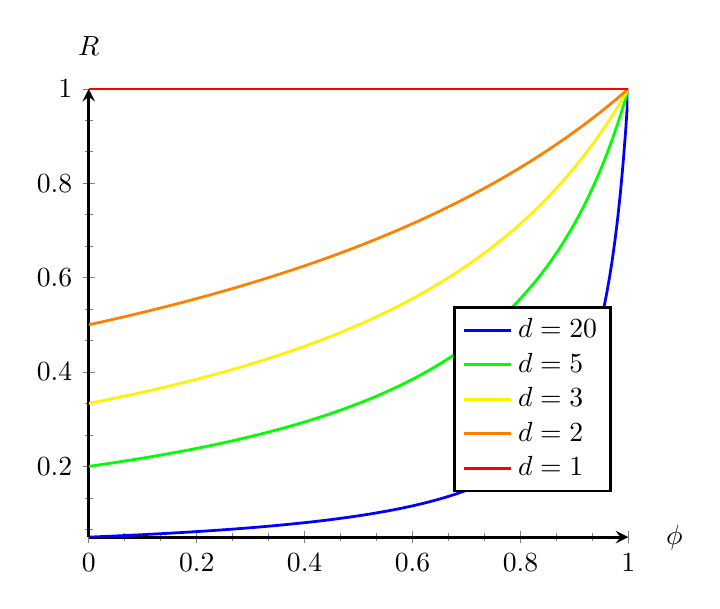
\begin{tikzpicture}
\begin{axis}[
ylabel={$R$},
xlabel={$\phi$},
domain=0:1,
samples=201,
legend entries={$d=20$,$d=5$,$d=3$, $d=2$,$d=1 $},
legend cell align=left,
minor tick num=2,
axis x line=bottom,
axis y line=left,
every axis x label/.style={
    at={(ticklabel* cs:1.05)},
    anchor=west,
},
every axis y label/.style={
    at={(ticklabel* cs:1.05)},
    anchor=south,
},
legend style={at={(0.97,0.1)},anchor=south east}
]
\addplot[blue]{1 /(20 - (20-1)* x)};
\addplot[green]{1 /(5 - (5-1)* x)};
\addplot[yellow]{1 /(3 - (3-1)* x)};
\addplot[orange]{1 /(2 - (2-1)* x)};
\addplot[red]{1 /(1 - (1-1)* x)};
\end{axis}
\end{tikzpicture}
\caption{ \textbf{Relatedness as a function of $d$ and $\phi$}. 
We assume a model of simultaneous infection. 
The figure is a plot of the relatedness against $\phi$ for several values of $d$ ranging from $1$ to $20$. 
We use the notation $\phi$ for the probability that two infecting nematode come from the same insect in the previous cycle. 
$d$ is the number of nematodes infecting the insect. 
If either the number of nematode is small or $\phi$ is large, the relatedness is close to one and the cooperation between bacteria is large}
\end{figure}
\subsection*{Consecutive infections}
In order to derive the relatedness under a model a consecutive infections, we first need to derive the probability of identity of bacteria inside an insect $\psic$. 
As previously, $\psic$ is the expected odds at which two randomly chosen bacteria (in the same insect) originate from the same nematode.  
Our assumptions is that the insect is infected by $2$ nematodes arriving successively. 
We assume nematodes arrive at times exponentially distributed of parameter $ \tau$. 
$\tau$ is a rate, and thus has the units of $[S^{-1}]$. 
We also assume the bacteria carried by the nematodes grew in a deterministic fashion at rate $\lambda$, and $\lambda$ has units of $[S^{-1}]$ also. 
Under these assumptions, we proved (see box 3) that $\psis$ is a decreasing function of the parameter $ \omega =\tau  \lambda^{-1}$, the ratio between the arrival rate of nematodes and the growth rate of bacteria:
\begin{equation}
   \psic (\omega)= 1- 2 \omega \mathrm{B}_{1/2}(1+\omega,1-\omega) \label{eqn:star2},
\end{equation}
where $\mathrm{B}_x(a,b)$ is the incomplete beta function:
\begin{align}
\mathrm{B}_x(a,b) = \int_0^x t^{a-1}(1-t)^{b-1} \ud t.
\end{align}
As previously, we use the notation $\nI$ for the total number of insects.
Let $Q_i$ be the probability of identity of genes from different bacteria, within the same insect ($\qw$) and in different insect ($\qb$). 
Here we consider the probability of identity in the infinite allele model, and let $u$ be the mutation rate.
The recursion equations for next generation identities $\qw '$ and $\qb '$ are the same as in the model of consecutive equation where $\psis$ is now $\psic $ and $\phi=\nI^{-1}$ since migration is homogeneous:
  \begin{subnumcases}{\hspace*{-1cm}}
      		\qw ' = (1-u)^2 \left[ \psic + \left( \dfrac{ \qw }{\nI}+\dfrac{\nI-1}{\nI} \qb \right) (1 -\psic) \right] \\
    		\qb ' = (1-u)^2 \left[ \dfrac{ \qw }{\nI}+\dfrac{\nI-1}{\nI} \qb \right].
  \end{subnumcases}
 At equilibrium, $\qw ' = \qw$ and $\qb ' =\qb$ and the recursion equations are:
  \begin{subnumcases}{\hspace*{-1cm}}
      		\qw = (1-u)^2 \left[ \psic + \left( \dfrac{\qw}{\nI}+\dfrac{\nI-1}{\nI} \qb \right) (1 -\psic) \right] \\
    		\qb = (1-u)^2 \left[ \dfrac{\qw}{\nI}+\dfrac{\nI-1}{\nI} \qb \right].
  \end{subnumcases}
 \begin{figure}[H]
\label{fig:RC}
\centering
\begin{tikzpicture}
\begin{axis}[
xlabel={$\omega$},
ylabel={$R$},
ymin=0.2, ymax=1,
legend cell align=left,
minor tick num=2,
axis x line=bottom,
axis y line=left,
every axis x label/.style={
    at={(ticklabel* cs:1.05)},
    anchor=west,
},
every axis y label/.style={
    at={(ticklabel* cs:1.05)},
    anchor=south,
},
legend style={at={(1,0.95)},anchor=north east}
] 
\addplot[purple] table[x index=0,y index=2,col sep=space] {data/4nematodes_randtime_randgrowth.txt};
\addlegendentry{Average value for d=4}
\addplot[blue] table[x index=0,y index=2,col sep=space] {data/3nematodes_randtime_randgrowth.txt};
\addlegendentry{Average value for d=3}
\addplot[green] table[x index=0,y index=3,col sep=space] {data/2nematodes_randtime_randgrowth.txt};
\addlegendentry{Lower estimate for d=2}
\addplot[red] table[x index=0,y index=4,col sep=space] {data/2nematodes_randtime_randgrowth.txt};
\addlegendentry{Upper estimate for d=2}
\addplot[black] table[x index=0,y index=1,col sep=space] {data/psic.dat};
\addlegendentry{Analytic function for d=2}
\addplot[black, no markers, ultra thin] coordinates {(0,0.5) (5,0.5)};
\addplot[black, no markers, ultra thin] coordinates {(0,0.333) (5,0.333)};
\addplot[black, no markers, ultra thin] coordinates {(0,0.25) (5,0.25)};
\end{axis}
\end{tikzpicture}
\caption{\textbf{Relatedness as a function of $d$ and $\omega$}. 
For the case of infection by two nematodes ($d=2$), and under the assumption of a deterministic growth of bacteria, the relatedness can be analytically derived as a function of $\omega$ (black solid line).
$\omega$ is the ratio between the arrival rate of nematodes and the growth rate of bacteria. 
To relief from these assumptions, we simulated infections for various number of nematodes and for values of the parameter $\omega$ from $0$ to $5$. 
In our simulation the growth of bacteria is stochastic. 
For two nematodes, the solid lines are the maximum (red) and minimum (green) estimate of $R$ over a thousand simulations. 
The average value of relatedness is also plotted for 3 (blue solid line) and 4 (purple solid line) nematodes. 
The relatedness decreases with the number of infecting nematodes. 
The relatedness also decreases with regard to $\omega$. 
That is to say the relatedness increases with regard to the growth rate of bacteria. 
Or equivalently the relatedness decreases with regard to the arrival rate of nematodes.}
\end{figure}
 This systems of equations can also be solved unambiguously and leads to the relatedness 
 \begin{align}
 R &= \dfrac{\qw - \qb }{1- \qb} \\
   &= \dfrac{(1-u)^2 \nI \psic}{\nI +(1-u)^2 \psic}.
 \end{align}
And thus by taking the limit for low mutation rate ($u \rightarrow 0$), the relatedness becomes:
 \begin{equation}
 R \simeq \dfrac{\psic}{1+ \dfrac{\psic}{\nI}}.
 \end{equation} 
Under the assumption of an important number of insects ($\nI \gg 1$), the relatedness is:
 \begin{equation}
 R \simeq \psic = 1- 2 \omega \mathrm{B}_{1/2}(1+\omega,1-\omega)
 \end{equation}
 The relatedness solely depends on the parameter $\omega$ for the case of infection by two nematodes.
  If the number of nematodes is greater than two, we expect the relatedness to depend solely on the number of nematodes and $\omega$, but we could not derive an analytic formula. 
  We remind that the formula was derived under strong assumptions, namely that only two nematodes infected the insect and that the bacteria growth is deterministic. 
  Thus we simulated the infection process process in order to take out this assumptions. 
  The simulations shows that the relatedness decreases with the number of infecting nematodes (see figure 4). 
  The relatedness also decreases with regard to $\omega$. That is to say the relatedness increases with regard to the growth rate of bacteria. 
  Or equivalently the relatedness decreases with regard to the arrival rate of nematodes, 
\section*{Discussion}
The parasitic life cycle of \Xeno and \Photo has a lot of influence on their relatedness, and thus on cooperation between bacteria. 
Under simplifying assumptions, we derive the candidate evolutionary strategy for phenotypic variation probability switch. 
This strategy is derived as a function of relatedness, a measure of closeness between species.  
The relatedness is subsequently derived as a function of demographic parameters, experimentally accessible.
Under tremendous effort, the phenotypic variation switch can be estimated experimentally, as well as the function $f$ measuring the success of nematodes with regard to the proportion of type I bacteria.
The model of simultaneous infection is adapted to evolution experiment. 
Indeed, there is no experimental barrier to manipulate parameters such as $d$ or $\phi$ in the laboratory, those the relatedness can be controlled under this framework. 
However, estimation if these parameters in the field seem a vain labor and this is the drawback of this model. 
The model of simultaneous infection is also adapted to evolution experiment. 
Indeed, if the birth rate ($\lambda$) of bacteria can be hardly controlled and thus considered as fixed, the infection rate by nematodes ($\tau$) can be controlled in laboratory experiment. 
The number of nematodes infecting the insects can also be controlled. 
Moreover, estimating the arrival rate of nematodes is accessible in field experiment, assuming one can lure nematodes to a trap containing the insect and measure the arrival times. 
Thus parameters estimation of this model are accessible, but this model likely does not reflect reality since we assume the migration process to be homogeneous. 

\Xnema and \Photo are invaluable models for studying cooperation at the bacteria level. 
Indeed phenotypic variation expresses the trade-off between a cooperator and a defector phenotype. 
The relatedness is also strongly depend on demographic and migration parameter, that can be tuned experimentally.
Finally, since nematodes are colonized by one or two bacteria, we expect the system to evolve fast and mutation can fix to the population quite quickly.
\section*{Acknowledgments}
I thank François Rousset and Jean-Baptiste Ferdy for their help and advise concerning this internship report and internship, as well as for insightful discussions. 
I am grateful to my laptop who coped my relentless bashing.
\bibliographystyle{plain}
\bibliography{References_none_mendeley,References}
\end{multicols}
\begin{boxframe}
\label{box_psi_simultaneous}
\begin{multicols}{2}
\textbf{Box 1. Proof of the equation \eqref{eqn:star}\\}
An insect is infected by $d$ nematodes. 
Each nematode $i$ ($ 1 \leq i \ d$) releases his bacteria inside the insect. 
The $d$ colonies of bacteria enter a stochastic growth process at time $t=0$.
In this context, $N_i(t)$ denotes the discrete random variable describing the population size of bacteria originating from the $i$th nematode, at time $t$. 
$N_+(t)=\sum_{i=0}^d N_i(t)$ denotes the discrete random variable describing the size of the whole population of bacteria at time $t$. 
The random variable $Z_i$ describes the frequency that two randomly chosen bacteria at time $t$ are originating from the $i$th nematode. 
By definition we have:
\begin{equation}
Z_i=\dfrac{N_i(t)(N_i(t)-1)}{N_+(t)( N_+(t)-1 ) }.
\end{equation} 
The expectation of the sum of $Z_i$ over all nematodes is thus $\psi (t)$, the probability 
that two randomly chosen bacteria originate from the same nematode. 
\begin{equation}
\psi(t) = \mathbb{E} \left[ \sum_{i=1}^d Z_i(t) \right] = \sum_{i=1}^d \mathbb{E}[ Z_i(t)]
\end{equation}
Thus we need to evaluate $\mathbb{E}[ Z_i(t)]$. 
The growth process is modeled as a discrete space, continuous time Markov process. Each bacterium has an constant birth rate $\lambda$ and they never die. Thus all bacteria is independent of one another. This model depicts an exponential growth. 
$k_i$ denote the number of bacteria initially contained in the $i$th nematode. The random variable $X_i(t)=N_i(t)-k_i$ is thus the number of births in the $i$th lineage. Under our model, 
$X_i(t)$ is a negative binomial\cite[p. 158]{cox1977theory}:
\begin{equation}
X_i(t) \sim \mathrm{NB} \left( k_i, e^{-\lambda t} \right) \iff
\end{equation}
\begin{equation}
\pr(X_i(t)=x)=\binom{x+k_i -1}{x} \left( e^{-\lambda t} \right)^{k_i} \left( 1-e^{-\lambda t} \right)^{x}.
\end{equation}
Consistently with previous notations, $k_+=\sum_{i=0}^d k_i$ is the total number of bacteria released initially by the $d$ nematodes. 
Equivalently $X_+(t)=N_+(t)-k_+$ is the total number of bacteria born. Since all $X_i(t)$ are independent of one another, $X_+(t)$ is also a negative binomial \cite{johnson2005univariate}:
\begin{equation}
 X_+(t)  \sim \mathrm{NB} \left( k_+, e^{-\lambda t} \right).
\end{equation}
Basic calculus leads to the distribution of $X_i(t)$ conditional on $ X_+(t)=x_+ $; this is a negative hypergeometric and independent of $e^{-\lambda t}$:
\begin{align}
\pr( X_i & (t) =x \vert X_+(t)=x_+ )  \nonumber \\ 
& = \dfrac{\displaystyle \binom{x+k_i-1}{x} \binom{x_+-x+k_+-k_i-1}{x_+-x}}{\displaystyle \binom{x_+ +k_+ -1}{x_+}}.
\end{align}
Leading to expectation for $X_i(t)(X_i(t)-1)$ conditional on $X_+(t)$:
\begin{align}
 \mathbb{E} [ X_i(t)& (X_i(t)-1) \vert X_+(t) ]  \nonumber \\
 &=\dfrac{k_i(k_i+1)}{k_+ (k_+ +1 )}X_+(t) ( X_+(t) -1 ).
\end{align}
And the expectation of $N_i(t)(N_i(t)-1)$ conditional on $N_+(t)$ is:
\begin{align}
 \mathbb{E} & [ N_i(t) (N_i(t)-1) \vert N_+(t) ]   \nonumber \\
 &=\dfrac{k_i(k_i+1) }{k_+ (k_+ +1)}N_+(t) ( N_+(t) -1 ) -\dfrac{2 k_i (k_+ - k_i) }{k_+ (k_+ +1)} N_+(t) .
\end{align}
Leading in turn to the expectation of $Z_i(t)$ conditional on $N_+(t)$.
\begin{align}
  \mathbb{E} [  Z_i(t)  & \vert N_+(t) ]  \nonumber \\
 &= \dfrac{k_i(k_i+1)}{k_+ (k_+ +1)}- \dfrac{2 k_i (k_+ -k_i)}{k_+ (k_+ +1)} \dfrac{1}{ N_+(t) -1  }.
\end{align}
By the law of conditional expectation:
\begin{align}
\mathbb{E}\left[ Z_i(t) \right] &= 
 \mathbb{E}\left[ \mathbb{E}\left[ \left. Z_i(t) \right\vert N_+(t) \right] \right]\\
 &=\dfrac{k_i(k_i+1)}{k_+ (k_+ +1 )}-\dfrac{2 k_i (k_+ -k_i)}{k_+ (k_+ +1 )}\mathbb{E}\left[\dfrac{1}{N_+(t)-1} \right] \\
 & =\dfrac{k_i(k_i+1)}{k_+ (k_+ +1 )}-2e^{-\lambda t}\dfrac{ k_i (k_+ -k_i)}{k_+ (k_+^2 -1 )}.
\end{align}
By summing $\mathbb{E}\left[ Z_i(t) \right]$ over all $i$, we evaluate the probability of identity $\psi(t)$:
\begin{equation}
\psi(t) =\dfrac{ k_+ + \sum_{i=1}^d k_i^2}{k_+ (k_+ +1)}  -2 e^{-\lambda t} \dfrac{ k_+^2-\sum_{i=1}^d k_i^2}{k_+ (k_+^2 -1) }.
\end{equation}
Under the assumption that the number of bacteria carried by each nematode is large enough ($k_i \gg 1$), $\psi(t)$ becomes independent of $t$ and does not depend anymore on 
 the bacteria growth rate:
 \begin{equation}
\psi \simeq \displaystyle \sum_{i=1}^d \left( \dfrac{ k_i}{\sum_{i=1}^d k_i} \right)^2.  
 \end{equation}
 The probability that two randomly chosen bacteria originate from the same nematode is approximately the sum over all nematodes of their squared initial proportions.
 \end{multicols}
\end{boxframe}
\begin{boxframe}
\label{box_relatedness}
\begin{multicols}{2}
\textbf{Box 2. Proof of the equation \eqref{eqn:relatedness_simultaneous}\\}
	\label{box:life_cycle_relatedness}
We use the notation $\phi$ for the probability that two infecting nematode come from the same insect in the previous cycle.
We use the notation $\nI$ for the total number of insects.
Let $Q_i$ be the probability of identity of genes from different bacteria, within the same insect ($\qw$) and in different insect ($\qb$). Here we consider the probability of identity 
in the infinite allele model, and let $u$ be the mutation rate.
 The recursion equations for next generation identities $\qw '$ and $\qb '$ are (see box X / or figure X): 
  \begin{subnumcases}{\hspace*{-1.cm}}
      		 \qw ' = (1-u)^2[\psis + (1 -\psis) ( \phi \qw + (1-\phi) \qb ]  \\
    		 \qb ' = (1-u)^2 \left[ \dfrac{ \qw }{\nI}+\dfrac{\nI-1}{\nI} \qb \right].
  \end{subnumcases}
 \begin{figure}[H]
	\centering  
  \includegraphics[width=\textwidth /2]{Figures/relatedness.png}\\
  \end{figure}
  At equilibrium, $\qw ' = \qw$ and $\qb ' =\qb$ and the recursion equations are:
  \begin{subnumcases}{\hspace*{-1cm}}
      		 \qw = (1-u)^2[\psis + (1 -\psis) ( \phi \qw + (1-\phi) \qb ] \\
    		 \qb = (1-u)^2 \left[ \dfrac{ \qw }{\nI}+\dfrac{\nI-1}{\nI} \qb \right].
  \end{subnumcases}
  This systems of equations can be solved unambiguously and leads to the relatedness
  \begin{align}
 R &= \dfrac{\qw - \qb }{ 1- \qb } \\
 &= \dfrac{ \psis (1-u)^2 }{ 1 - (1-u)^2 \phi (1- \psis )+(1-u)^2 / \nI } .
 \end{align}
And thus by taking the limit for low mutation rate ($u \rightarrow 0$), the relatedness becomes:
 \begin{equation}
 R \simeq \dfrac{ \psis  }{ 1 - \phi (1- \psis )+1 / \nI }.
 \end{equation} 

 \end{multicols}
\end{boxframe}
\begin{boxframe}
\label{box_psi_consecutive}
\begin{multicols}{2}
\textbf{Box 3. Proof of  the formula \eqref{eqn:star2}\\}
We derive an analytic formula for $\psic$ for two nematodes arriving successively. 
We assume the first nematode arrive at time $T$ before the second (and last) nematode, where $T\sim \exp ( \tau)$. 
We also assume assume each nematode carries the same number of bacteria, $k \gg 1$. 
And finally, we assume the bacteria carried by the nematodes grew in a deterministic fashion at rate $\lambda$. 
Under all these assumptions, the number of bacteria in the insect when the second nematode arrives is the random variable $k e^{\lambda  T}+k$. 
Where $k e^{\lambda  T}$ bacteria are from the first one arrived and $k$ are from the second one.\\ 
  Since $k \gg 1$, the random variable $k e^{\lambda  T} $ is always far greater than $1$. 
  Thus we can make use of the equation \eqref{eqn:star} to derive $\psic$:
  \begin{align}
  \psic  &=\mathbb{E} \left[ \left( \dfrac{ k e^{\lambda T}}{k+ke^{\lambda T}} \right)^2+\left( \dfrac{k}{k+ke^{\lambda T}} \right)^2 \right] \\
  &=\mathbb{E} \left[ \left( \dfrac{ e^{\lambda T}}{1+e^{\lambda T}} \right)^2+\left( \dfrac{1}{1+e^{\lambda T}} \right)^2 \right] \\
  &=\int_0^\infty \left( \left( \dfrac{ e^{\lambda t}}{1+e^{\lambda t}} \right)^2 + \left( \dfrac{1}{1+e^{\lambda t}} \right)^2 \right) \tau e^{ -\tau t } \ud t.
  \end{align}
  The evaluation of this integral is not straightforward. 
  Instead we derive the cumulative distribution function $F_1(p)$ and $F_2(p)$ of $\dfrac{ e^{\lambda T}}{1+e^{\lambda T}}$ and $\dfrac{ 1}{1+e^{\lambda T}}$ respectively.
  \begin{align}
  F_1(p) &= \pr \left(\dfrac{e^{\lambda T}}{1+e^{\lambda T}} \leq p\right)= \pr \left(T \leq \lambda^{-1} \mathrm{ln}\left( \dfrac{p}{1-p} \right) \right) \nonumber \\
  &= 1-(1-p)^{\omega} p^{-\omega} \text{ for } 1/2 \leq p \leq 1,
  \end{align} 
  where $\omega=\tau / \lambda$.
  \begin{align}
  F_2(p) &= \pr \left(\dfrac{1}{1+e^{\lambda T}} \leq p\right) = \pr \left(T \geq \lambda^{-1} \mathrm{ln}\left( \dfrac{1-p}{p} \right) \right) \nonumber \\
  &= (1-p)^{-\omega} p^\omega \text{ for } 0 \leq p \leq 1/2.
  \end{align}
  Hence the the probability density function $f_1(p)$ and $f_2(p)$ are:
  \begin{align}
  f_1(p) &= \dfrac{ \ud F_1(p) }{ \ud p} =  \omega (1-p)^{\omega-1} p^{-\omega-1}  \text{ for } 1/2 \leq p \leq 1\\
  f_2(p) &= \dfrac{ \ud F_2(p) }{ \ud p} =  \omega (1-p)^{-\omega-1} p^{\omega-1} \text{ for } 0 \leq p \leq 1/2.
  \end{align}
  And 
  \begin{align}
  \psic (\omega)&= \int_{1/2}^{1} p^2 f_1(p) \ud p + \int_{0}^{1/2} p^2 f_2(p) \ud p \\
  &= 1 -2  \omega \int_{0}^{1/2}  (1-x)^{-\omega} x^{\omega}  \ud x \\
  &= 1- 2 \omega \mathrm{B}_{1/2}(1+\omega,1-\omega). 
  \end{align}
  where $\mathrm{B}_x(a,b)$ is the incomplete beta function:
\begin{align}
\mathrm{B}_x(a,b) = \int_0^x t^{a-1}(1-t)^{b-1} \ud t.
\end{align}
  Thus the probability of identity is solely dependent on one parameter, $\omega$, the ratio between arrival rate of nematodes and growth rate of bacteria. 
 \end{multicols}
\end{boxframe}
\end{document}

% \begin{tikzpicture}
%\begin{axis}[
%view={-45}{45},
%colorbar horizontal,
%colormap/temp,
%title={$R \simeq \dfrac{ \psi  }{ 1 - \phi (1- \psi )}$},
%xlabel={$\psi$},
%ylabel={$\phi$},
%]
%\addplot3[
%surf,
%domain=0:1,
%domain y=0:1,
%shader=faceted interp,
%draw=black,
%]
%{x /(1 - (1 - x)* y)};
%\end{axis}
%\end{tikzpicture}

%\begin{figure*}[hbt!]
%	  \centering
%	  \label{fig:fitness}
%       \includegraphics[width=14.0cm]{Figures/fitness.png}\\
%		\caption{\textbf{ The bacteria cooperation along the life cycle.} 
%The life cycle is the same as in figure 1 but we introduce phenotypic variation, namely type I and II. 
%Type I are more virulent toward the insect, support nematode growth and development, kill off unwanted guests but cannot associate with the nematode. 
%On the other hand, type II only associate to the nematode. 
%The phenotype under investigation, $z_\bullet$ is the probability for one bacteria to switch from type I to type II. 
%$z_0^{\mathrm{R}}$ is the proportion of type II in the insect, and the success of nematodes migrating out of the insect is $f(1- z_0^{\mathrm{R}})$. 
%The average success of nematodes migrating out of all insects is $f(1- \bar{z})$. 
%Thus the fitness of a focal bacterium is $z_\bullet f(1- z_0^{\mathrm{R}}) [f(1- \bar{z} ) z_0^{\mathrm{R}}]^{-1}$. 
%We assume all bacteria switch back from type II to I during the soil dwelling stage.}
%\end{figure*}
